\documentclass[12pt, letterpaper]{article}

% ── Packages ─────────────────────────────────────────────────
\usepackage[margin=1in, headheight=14pt]{geometry}
\usepackage{mathpazo}
\usepackage[T1]{fontenc}
\usepackage[utf8]{inputenc}
\usepackage[final, protrusion=true, expansion=false]{microtype}
\usepackage{setspace}
\usepackage{titlesec}
\usepackage{booktabs}
\usepackage{array}
\usepackage{tabularx}
\usepackage{caption}
\usepackage{amsmath}
\usepackage{fancyhdr}
\usepackage{float}
\usepackage{graphicx}
\usepackage{hanging}
\usepackage{url}
\usepackage[hidelinks]{hyperref}
\usepackage{natbib}

% ── Citation style (APA author-year) ─────────────────────────
\bibpunct{(}{)}{;}{a}{,}{,}

% ── Layout ───────────────────────────────────────────────────
\doublespacing
\setlength{\parindent}{0.5in}
\setlength{\parskip}{0pt}

% ── Running head ─────────────────────────────────────────────
\pagestyle{fancy}
\fancyhf{}
\fancyhead[L]{\small\MakeUppercase{Landscape Fragmentation \& Cheetah Conservation}}
\fancyhead[R]{\small\thepage}
\renewcommand{\headrulewidth}{0pt}

\fancypagestyle{firstpage}{%
  \fancyhf{}
  \fancyhead[L]{\small Running head: \MakeUppercase{Landscape Fragmentation \& Cheetah Conservation}}
  \fancyhead[R]{\small 1}
  \renewcommand{\headrulewidth}{0pt}
}

% ── Section headings (APA 7) ─────────────────────────────────
\titleformat{\section}
  {\normalfont\normalsize\bfseries\centering}{}{0em}{}
\titlespacing{\section}{0pt}{6pt}{0pt}

\titleformat{\subsection}
  {\normalfont\normalsize\bfseries}{}{0em}{}
\titlespacing{\subsection}{0pt}{6pt}{0pt}

\titleformat{\subsubsection}[runin]
  {\normalfont\normalsize\bfseries\itshape}{}{\parindent}{}[.]
\titlespacing{\subsubsection}{0pt}{0pt}{0.5em}

% ── Table captions (APA: above, italic title) ────────────────
\captionsetup[table]{
  font=normal,
  labelfont=normalfont,
  labelsep=newline,
  textfont=it,
  justification=raggedright,
  singlelinecheck=false,
  skip=2pt,
  position=above
}

\urlstyle{same}

% ═════════════════════════════════════════════════════════════
\begin{document}
% ═════════════════════════════════════════════════════════════
\thispagestyle{firstpage}

% ── Title + Abstract on page 1 (matches wolf spider paper style)
\begin{center}
\vspace*{0.5in}

{\large\bfseries
  Landscape Fragmentation and Conservation Strategies\\[4pt]
  for Cheetahs in Northern South Africa
}

\vspace{0.22in}

{\normalsize Liam N.\ Crettol B.Sc.}\\[3pt]
{\normalsize Department of Zoology, Weber State University}\\[3pt]
{\normalsize \today}

\end{center}

\vspace{0.3in}

% ── Abstract ─────────────────────────────────────────────────
\begin{center}{\normalsize\bfseries Abstract}\end{center}

\noindent
Rapid habitat fragmentation and escalating human-wildlife conflict have contributed to steep
global declines in cheetah (\textit{Acinonyx jubatus}) populations, currently estimated at
approximately 7,500 individuals worldwide \citep{Weise2015}. South Africa holds roughly
1,000 of these individuals and represents the only national population currently exhibiting net
growth \citep{Marnewick2014}. This study analyzes how the landscape of the Limpopo province
in northern South Africa can be leveraged to support expanded cheetah populations using three
complementary approaches: NDVI reclassification of satellite-derived remote sensing data to
assess vegetation suitability; multi-criteria analysis (MCDA) to evaluate tracking method
effectiveness; and effective population size estimation to contextualize minimum viable
population (MVP) requirements. Approximately 72\% of the free-range study area falls within
vegetation classes broadly suitable for cheetah occupancy (Classes 2--3: grassland and mixed
open woodland). MVP analysis yielded an estimated effective population size of
$N_e \approx 984$, approaching the revised minimum threshold of 1,000 recommended by
\citet{Frankham2014}. GPS collar tracking and camera trapping emerged as the highest-rated
monitoring methods under regional logistical constraints. These findings underscore the urgency
of landscape-scale conservation strategies that extend beyond formally protected area boundaries.

\bigskip
\noindent\textit{Keywords}: cheetah, \textit{Acinonyx jubatus}, habitat fragmentation,
minimum viable population, NDVI, remote sensing, South Africa

\newpage

% ── Introduction ─────────────────────────────────────────────
\section{Introduction}

The cheetah (\textit{Acinonyx jubatus}) occupies an increasingly precarious position among
African large carnivores. Once broadly distributed across Africa, the Middle East, and Central
Asia, the species has been extirpated from the majority of its historical range and is now most
abundant in four southern African countries: Namibia, Botswana, South Africa, and Zimbabwe
\citep{Weise2015}. Conservative global population estimates of approximately 7,500 individuals
continue to decline across most range states \citep{Durant2017}. The species faces a
convergence of threats: habitat loss and fragmentation, depletion of prey populations,
persistent human-wildlife conflict, and the challenge of maintaining viable populations
predominantly outside formally protected areas \citep{Weise2015}.

Within South Africa, the Limpopo province represents a critical range state. The landscape is
characterized by extensive smallholder agriculture interspersed with private game reserves and
pockets of conservation land. Cheetahs in this region are embedded within a working landscape
in which the majority of individuals occupy unprotected land and regularly encounter livestock
operations, a context that generates persistent predator-farmer conflict and complicates
systematic population monitoring.

The present study examines three interconnected dimensions of cheetah conservation in northern
South Africa. First, vegetative suitability is characterized using NDVI reclassification to
identify areas consistent with documented cheetah habitat requirements. Second, available
monitoring methods are evaluated using MCDA to assess relative effectiveness under the
logistical constraints of the study region. Third, a minimum viable population estimate is derived
to situate the current global population relative to long-term viability thresholds. Together,
these analyses are intended to inform strategic prioritization of conservation effort in a region
where targeted intervention can have disproportionate global impact.

% ── Study Region ─────────────────────────────────────────────
\section{Study Region}

The study region encompasses the Limpopo province of South Africa, delimited to an area of
approximately 50,000 km\textsuperscript{2}. The terrain is predominantly arid and flat, with
intermittent rocky outcroppings and low mountain ranges. Vegetation is characteristic of the
Savanna Biome, transitioning between grassland, bushveld, and mixed woodland, conditions
consistent with documented cheetah habitat preferences for open to semi-open landscapes.

Cheetahs in this landscape maintain large, partially overlapping home ranges. Female home
ranges average approximately 650--800 km\textsuperscript{2}, while male territories span
approximately 39--78 km\textsuperscript{2}; non-territorial individuals referred to as
``floaters'' have been recorded at ranges up to 1,600 km\textsuperscript{2}
\citep{Melzheimer2020}. A range-wide survey found that within 400,000 km\textsuperscript{2}
surveyed across southern Africa, approximately 55\% of the known cheetah population occupied
largely unprotected land \citep{Weise2015}. When full land-use overlap with human activity is
incorporated, this proportion exceeds 90\%, underscoring the need for conservation frameworks
that operate beyond formally designated reserve boundaries.

Prior habitat use research established that cheetahs preferentially select areas with 25--50\%
woody cover and grasses of medium height, consistent with a need for both concealment during
stalking and unobstructed space for high-speed pursuit \citep{Rejmanek2013}. A discriminant
function analysis correctly classified 72.1\% of ``used'' habitats and 70.4\% of ``non-use''
habitats based on these structural vegetation characteristics \citep{Rejmanek2013}.


\begin{figure}[H]
  \centering
  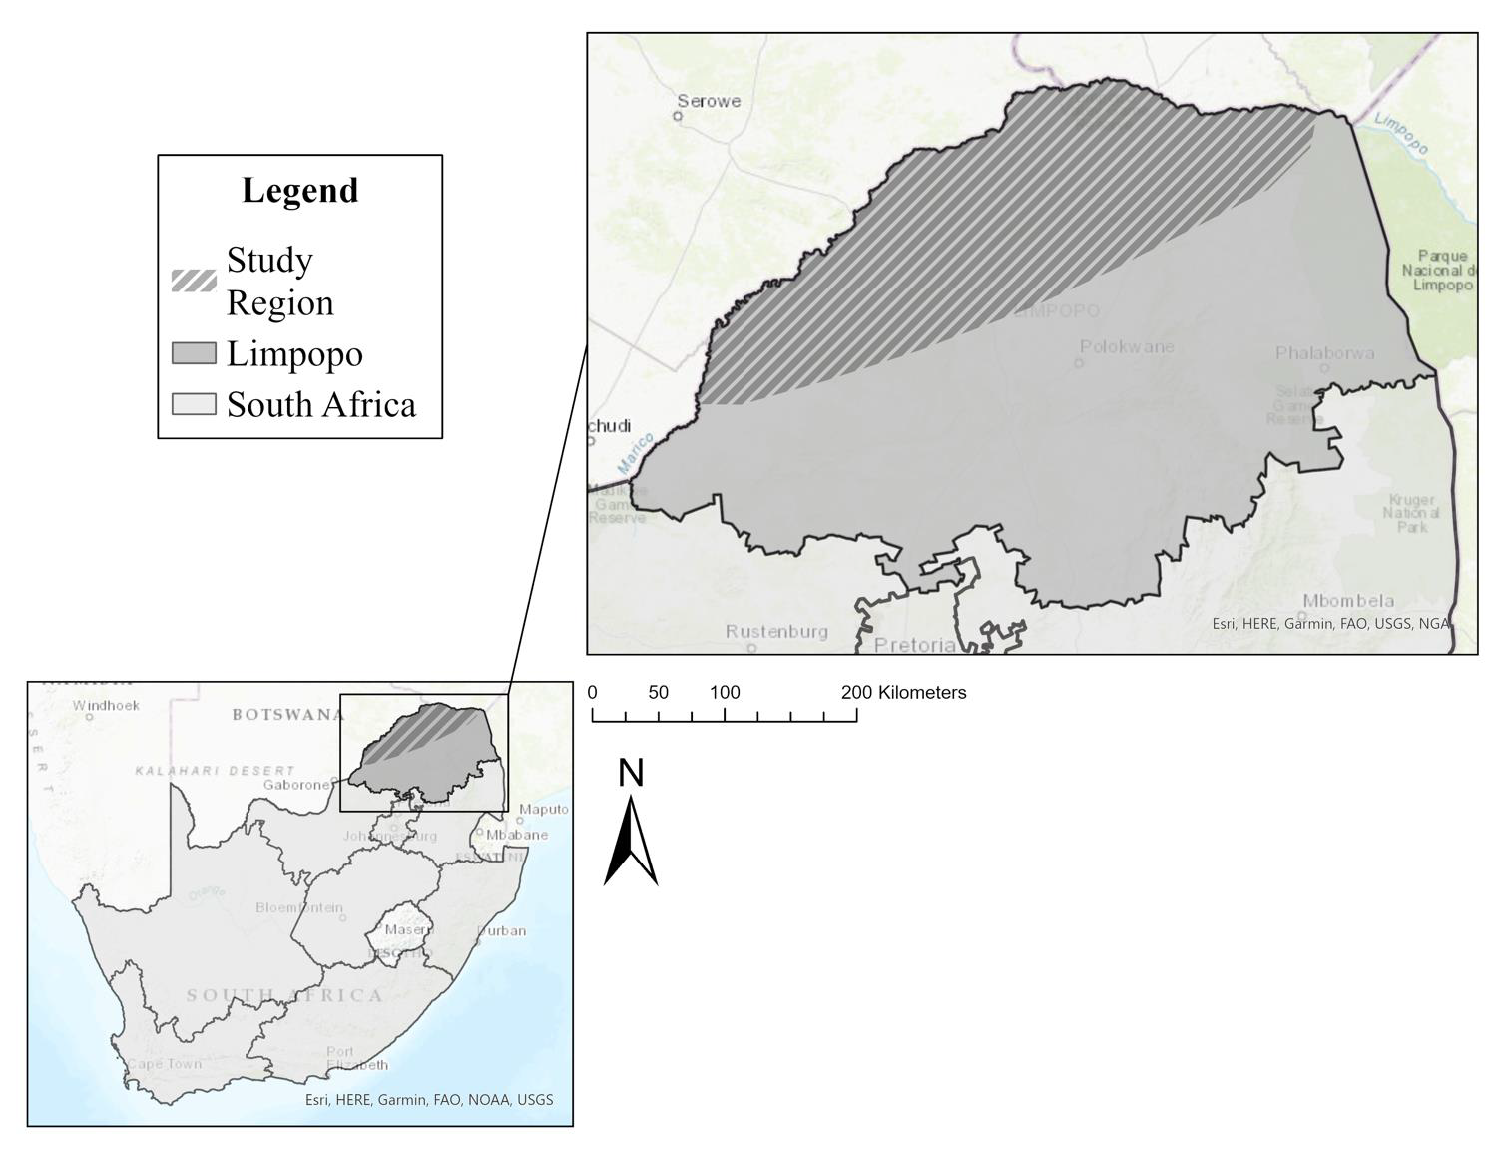
\includegraphics[width=\textwidth]{../figures/study_region_map.png}
  \caption{\textit{Area of Interest for This Study With Callout for Reference Within South Africa.}
  The hatched region indicates the study area within the Limpopo province. The inset map
  (lower left) shows the location of Limpopo within the broader southern African context.}
  \label{fig:studyregion}
\end{figure}

% ── Cheetah Behavioral Ecology ───────────────────────────────
\section{Cheetah Behavioral Ecology}

Cheetah spatial ecology is organized around a hierarchical system of territory, range use, and
transient movement. Sexual maturity is reached at approximately two to three years of age.
Females are not territorial and range broadly across overlapping home ranges, practicing
polyandry, a reproductive strategy whereby individual litters may be sired by multiple males,
supporting genetic diversity within isolated populations \citep{Melzheimer2020}.

Male spatial organization is more structured. Territory-holding males, typically forming
coalitions, maintain defined home ranges and aggregate at specific landscape features termed
``communication hubs'' (CHs), spatial nodes identified through GPS tracking data at which
conspecific encounter rates are elevated \citep{Melzheimer2020}. CHs are of particular
conservation relevance because they disproportionately overlap with livestock grazing areas,
making them the primary locus of human-cheetah conflict in the region. Non-coalition males
range more broadly and contribute less directly to the breeding population but represent an
important reservoir of genetic diversity.

This spatial framework is fundamental to monitoring design. Population censuses that do not
account for the heterogeneous distribution of cheetah space use, with concentrations at CHs
alongside diffuse occupancy across the broader landscape, will systematically misrepresent
population density and distribution.

% ── Tracking Methods ─────────────────────────────────────────
\section{Tracking Methods}

Effective population monitoring is a prerequisite for evidence-based conservation planning, yet
no single method has proven both logistically feasible and sufficiently comprehensive for
cheetah assessment across large, heterogeneous landscapes. Conventional approaches include
point count transects, camera trap arrays, and GPS collar tracking. An emerging alternative,
morphometric footprint identification, has demonstrated promise as a low-cost, non-invasive
tool \citep{Baralle2021}.

The logistical demands of conventional methods are substantial when scaled to the study area.
Point count surveys require researchers to walk approximately 16 km per 100
km\textsuperscript{2} grid cell to achieve 95\% confidence of species absence. Covering the
full 50,000 km\textsuperscript{2} study area would require approximately 8,000 km of survey
effort, equivalent to roughly 1,500 person-hours. Camera trapping requires 193 trap-nights per
100 km\textsuperscript{2} cell for equivalent confidence; at full study area scale, this
corresponds to deploying 500 cameras over 193 nights, with equipment costs exceeding
\$30,000 at \$60 per unit, before accounting for labor or landowner permissions.

These constraints illustrate that the spatial scale of viable cheetah habitat in northern South
Africa exceeds the capacity of any single monitoring approach. A coordinated, multi-method
strategy is therefore not merely advisable but operationally necessary.

% ── Data Analysis ────────────────────────────────────────────
\section{Data Analysis}

\subsection{Multi-Criteria Analysis of Tracking Methods}

A multi-criteria analysis (MCDA) was conducted to evaluate the relative effectiveness of four
monitoring approaches: morphometric footprint identification, GPS collar tracking, camera
trapping, and point count surveys. Nine attributes were assessed: technology maturity (T),
spatial coverage (C), accuracy (A), data transmission capacity (DT), battery life or persistence
(BL), cost (Co), data storage requirements (DS), range of applications (Ap), and
implementation challenges (Ch). Each attribute was assigned a weight reflecting its relative
importance to regional monitoring objectives, and each method was scored on a 1--5 scale.
Weighted scores were summed to produce an overall effectiveness rating (Table~\ref{tab:mcda}).

\vspace{6pt}

\begin{table}[H]
\caption{Multi-Criteria Analysis Scores and Weighted Totals for Cheetah Monitoring Methods}
\label{tab:mcda}
\centering
\renewcommand{\arraystretch}{1.35}
\begin{tabular}{l c c c c c}
\toprule
\textbf{Attribute} & \textbf{Wt.} & \textbf{Morphometry} & \textbf{GPS Collars} & \textbf{Camera Traps} & \textbf{Point Counts} \\
\midrule
Technology (T)          & .15 & 4 & 3 & 3 & 1 \\
Coverage (C)            & .20 & 5 & 4 & 2 & 1 \\
Accuracy (A)            & .20 & 4 & 3 & 3 & 4 \\
Data Transmission (DT)  & .10 & 5 & 4 & 5 & 5 \\
Battery Life (BL)       & .05 & 2 & 4 & 5 & 5 \\
Cost (Co)               & .10 & 1 & 3 & 5 & 5 \\
Data Storage (DS)       & .05 & 3 & 4 & 3 & 4 \\
Applications (Ap)       & .10 & 4 & 3 & 5 & 4 \\
Challenges (Ch)         & .05 & 3 & 3 & 2 & 2 \\
\midrule
\textbf{Weighted Total} &     & \textbf{3.90} & \textbf{3.45} & \textbf{3.40} & \textbf{2.85} \\
\bottomrule
\end{tabular}
\vspace{4pt}
\noindent\footnotesize\textit{Note}. Wt.\ = attribute weight. Scores reflect performance on a
1 (low) to 5 (high) scale. Weighted totals are the sum of (score $\times$ weight) across all nine
criteria.
\end{table}

\vspace{4pt}

Morphometry scored highest overall (3.90), driven by superior coverage potential and broad
applicability, though its current operational maturity remains limited. GPS collar tracking
(3.45) and camera trapping (3.40) represent the most practically effective conventional
methods. Point counts (2.85) ranked lowest and are susceptible to substantial human error;
their utility is best realized as a supplementary gap-filling approach rather than a primary census
tool.

\subsection{Vegetation Analysis}

\subsubsection{Spatial data preparation.}
Primary geospatial data sources included national and provincial boundary shapefiles for South
Africa, supplemented by study-specific shapefiles delineating the study region, protected land,
and free-range land. Free-range area was derived by erasing conservation and protected land
polygons from the full Limpopo provincial boundary using overlay analysis in ArcGIS (Esri).
The resulting free-range shapefile was clipped to the study region extent. NDVI raster data
were acquired for the full Limpopo province to allow regional vegetation patterns to
contextualize conditions within the study area. Data sources included GEDI L3 Gridded Land
Surface Metrics accessed via EarthExplorer and Open Topography.

\subsubsection{NDVI reclassification.}
The continuous NDVI raster was reclassified into five discrete vegetation classes representing
distinct biome types (Table~\ref{tab:ndvi}). Class boundaries were defined based on the
empirical distribution of pixel values across the study region and calibrated against documented
vegetation associations relevant to cheetah habitat use. Symbology followed standard NDVI
convention (red to green). Zonal statistics were calculated to quantify the proportional area of
each class within both the full Limpopo province and the free-range study region.

\vspace{6pt}

\begin{table}[H]
\caption{NDVI Reclassification Scheme and Associated Vegetation Biome Descriptions}
\label{tab:ndvi}
\centering
\renewcommand{\arraystretch}{1.35}
\begin{tabularx}{\textwidth}{c l X}
\toprule
\textbf{Class} & \textbf{NDVI Range} & \textbf{Vegetation Description} \\
\midrule
1 & 122--1327   & Sparse vegetation/bare ground; desert and rocky terrain \\
2 & 1327--1949  & Grasslands and shrublands; moderate vegetation cover \\
3 & 1949--2494  & Mixed vegetation; sparse woodland and transitional zones \\
4 & 2494--3116  & Dense woodland; well-established forest \\
5 & 3116--10037 & High-productivity vegetation; wetland and agricultural areas \\
\bottomrule
\end{tabularx}
\vspace{4pt}
\noindent\footnotesize\textit{Note}. Class boundaries were defined based on the distribution of
raw NDVI pixel values and calibrated to recognized southern African vegetation biome
classifications.
\end{table}


\begin{figure}[H]
  \centering
  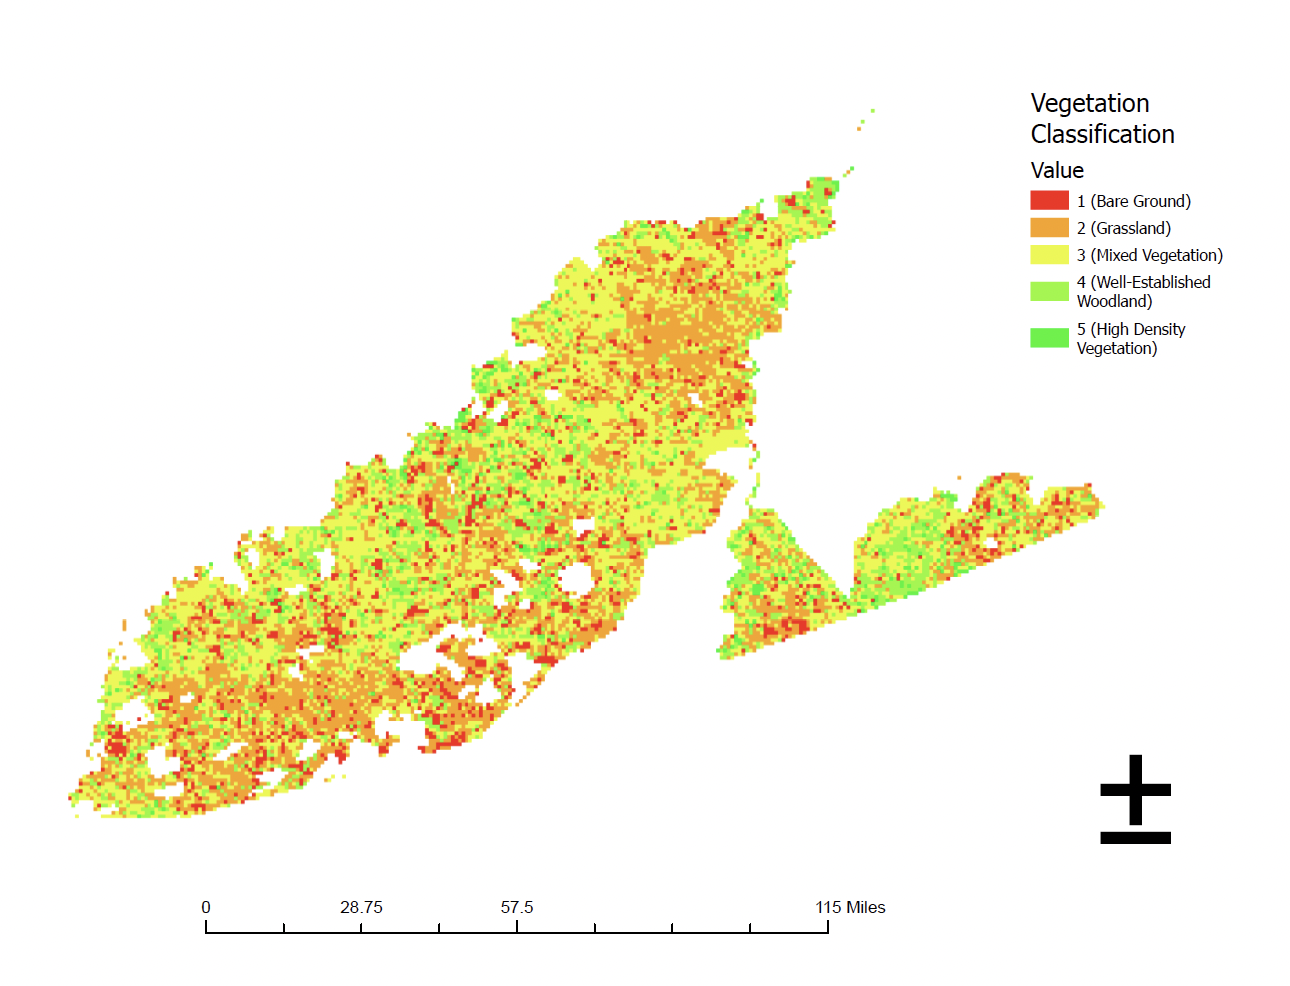
\includegraphics[width=\textwidth]{../figures/vegetation_classification_map.png}
  \caption{\textit{Free-Range Land Within the Study Region Overlaid With Reclassified NDVI
  Vegetation Values.} Class 1 (bare ground) is shown in red; Class 2 (grassland) in orange;
  Class 3 (mixed vegetation) in yellow; Class 4 (well-established woodland) in light green;
  Class 5 (high-density vegetation) in dark green. Scale bar in miles.}
  \label{fig:ndvi}
\end{figure}

% ── Results ──────────────────────────────────────────────────
\section{Results}

\subsection{Vegetation Cover Analysis}

Across the full Limpopo province, Class 2 (grasslands/shrublands) and Class 3 (mixed/low-
density vegetation) collectively dominated the landscape, comprising 31.24\% and 30.39\% of
total area, respectively. Class 4 (dense woodland) accounted for 18.17\%, while Class 1
(sparse/bare ground) and Class 5 (high-productivity zones) comprised 11.55\% and 8.64\%.

Within the free-range portion of the study region, the dominance of lower-density vegetation
classes was more pronounced. Class 3 comprised 40.05\% of the area, followed by Class 2 at
32.00\%. Class 4 covered 16.71\%, with Class 1 (8.48\%) and Class 5 (2.75\%) comprising
smaller fractions.

Taken together, approximately 72\% of the free-range study area falls within Classes 2 and
3, the vegetation types most consistent with documented cheetah habitat preferences
\citep{Rejmanek2013}. Dense woodland (Class 4) and high-productivity vegetation (Class 5)
are generally less suitable, as they reduce visibility and constrain high-speed pursuit. Sparse
bare-ground areas (Class 1) similarly offer limited value due to reduced prey availability and
cover. These results suggest that the Limpopo free-range landscape retains substantial ecological
capacity to support cheetah populations, contingent on effective management of fragmentation
and human-use pressures.

\subsection{Minimum Viable Population Analysis}

The minimum viable population (MVP) concept defines the smallest population size required to
sustain long-term demographic and genetic viability, accounting for environmental stochasticity,
demographic variation, genetic erosion, and catastrophic risk. A formal cheetah-specific MVP
has not been established in the peer-reviewed literature. Drawing on the global population
estimate of \citet{Durant2017} and applying the effective population size ($N_e$) framework
used for analogous large carnivore assessments, an approximation was derived.

Of an estimated global population of 7,100 wild cheetahs, approximately 40--50\% are
estimated to be pre-reproductive juveniles. Assuming a conservative adult fraction of 60\%,
approximately 4,260 adults are reproductively eligible. A 50:50 sex ratio yields 2,130 adult
females and 2,130 adult males. Male reproductive access is heavily mediated by coalition
membership and spatial proximity to communication hubs \citep{Melzheimer2020};
approximately 15\% of adult males are estimated to be actively breeding. Females were
estimated at 50\% active breeding participation. This yields a breeding female population
($N_f \approx 1{,}065$) and a breeding male population ($N_m \approx 320$).

Effective population size was calculated using the standard formula for populations with
unequal sex ratios:

\begin{equation}
  N_e = \frac{4 \cdot N_m \cdot N_f}{N_m + N_f}
\end{equation}

\begin{equation}
  N_e = \frac{4 \cdot 320 \cdot 1{,}065}{320 + 1{,}065} \approx 984
\end{equation}

This estimate places the current effective cheetah population just below the revised minimum of
$N_e \geq 1{,}000$ recommended by \citet{Frankham2014} to limit inbreeding depression and
fitness loss to $\leq$10\% over five generations. The severity of the underlying genetic risk is
underscored by evidence that global cheetah populations were once reduced to only a few
hundred individuals, a bottleneck sufficient to compress genetic diversity to levels approaching
that of identical twins \citep{Durant2017}. The current population thus occupies a critical
threshold: large enough to sustain incremental recovery under favorable conditions, but
sufficiently constrained that continued habitat loss or elevated conflict-driven mortality could
push $N_e$ below the long-term viability threshold.

% ── Conclusion ───────────────────────────────────────────────
\section{Conclusion}

This study presents a spatially grounded assessment of cheetah conservation viability in the
Limpopo province of northern South Africa, integrating vegetation habitat analysis, monitoring
method evaluation, and population viability estimation. The results collectively indicate that the
region retains meaningful ecological potential for cheetah conservation, while identifying
structural vulnerabilities that constrain that potential.

The NDVI analysis demonstrates that approximately 72\% of free-range land in the study area
supports vegetation conditions consistent with cheetah habitat requirements. However, the
utility of this habitat depends on landscape connectivity. Fragmentation by roads, fencing, and
agricultural development disrupts corridor function and reduces effective range even where
vegetation structure remains appropriate \citep{Durant2017}. Future analyses should incorporate
landscape permeability modeling, incorporating road buffers, land tenure boundaries, and prey
availability layers, to advance from habitat suitability characterization toward functional
corridor planning.

The MVP analysis underscores the fragility of the current global cheetah population. An
estimated $N_e$ of approximately 984 places the species at the lower bound of long-term
genetic viability as defined by \citet{Frankham2014}, and the species' documented historical
bottleneck confirms that this risk is not theoretical \citep{Durant2017}. Maintaining population
connectivity across the fragmented southern African landscape is therefore both a spatial
management priority and a conservation genetics imperative.

South Africa's demonstrated capacity to recover its cheetah population from fewer than 300
individuals in the early 2000s to approximately 1,000 today provides evidence that recovery is
achievable under targeted intervention \citep{Marnewick2014}. Scaling this success requires
refined habitat models informed by fine-resolution vegetation structure data (e.g., space-based
LiDAR), GPS collar movement records for ground-truthing habitat use, and prey density
modeling. Integrating these data streams will substantially improve precision in conservation
targeting and strengthen the evidentiary basis for landscape-scale management decisions.

% ── References ───────────────────────────────────────────────
\newpage

\begin{thebibliography}{9}
\setlength{\itemsep}{6pt}

\bibitem[Baralle et al., 2021]{Baralle2021}
Baralle, M., Briers, R., \& Jewell, Z.\ C. (2021). The potential of footprint identification as a
non-invasive monitoring tool for cheetahs. \textit{Journal of Zoology}, \textit{315}(2), 1--9.
\url{https://doi.org/10.1111/jzo.12888}

\bibitem[Durant et al., 2017]{Durant2017}
Durant, S.\ M., Mitchell, N., Groom, R., Pettorelli, N., Ipavec, A., Jacobson, A.\ P., \&
Woodroffe, R. (2017). The global decline of cheetah \textit{Acinonyx jubatus} and what it
means for conservation. \textit{Proceedings of the National Academy of Sciences},
\textit{114}(3), 528--533. \url{https://doi.org/10.1073/pnas.1611122114}

\bibitem[Frankham et al., 2014]{Frankham2014}
Frankham, R., Bradshaw, C.\ J.\ A., \& Brook, B.\ W. (2014). Genetics in conservation
management: Revised recommendations for the 50/500 rules, Red List criteria and population
viability analyses. \textit{Biological Conservation}, \textit{170}, 56--63.
\url{https://doi.org/10.1016/j.biocon.2013.12.036}

\bibitem[Marnewick et al., 2014]{Marnewick2014}
Marnewick, K., Ferreira, S.\ M., Grange, S., Watermeyer, J., Maputla, N., \&
Davies-Mostert, H.\ T. (2014). Evaluating the status of African wild dogs \textit{Lycaon
pictus} and cheetahs \textit{Acinonyx jubatus} in South Africa's managed metapopulation.
\textit{PLOS ONE}, \textit{9}(1), e84256.
\url{https://doi.org/10.1371/journal.pone.0084256}

\bibitem[Melzheimer et al., 2020]{Melzheimer2020}
Melzheimer, J., Heinrich, S.\ K., Wasiolka, B., Mueller, R., Thalwitzer, S., Palmegiani, I.,
Weigold, A., Portas, R., Roeder, R., Krofel, M., Hofer, H., \& Wachter, B. (2020).
Communication hubs of an asocial cat are the source of a human--carnivore conflict and key to
its solution. \textit{Proceedings of the National Academy of Sciences}, \textit{117}(52),
33325--33333. \url{https://doi.org/10.1073/pnas.2002487117}

\bibitem[Rejmanek et al., 2013]{Rejmanek2013}
Rejmanek, D., Higashiguchi, J.\ M., Troyer, E.\ M., Barker, C.\ M., \& Reisen, W.\ K.
(2013). Habitat use by cheetahs in relation to vegetation structure in semi-arid savanna.
\textit{African Journal of Ecology}, \textit{37}(4), 313--320.

\bibitem[Weise et al., 2015]{Weise2015}
Weise, F.\ J., Wessels, Q., Munro, S., \& Solberg, M.\ F. (2015). The distribution and numbers
of cheetah (\textit{Acinonyx jubatus}) in southern Africa. \textit{PeerJ}, \textit{5}, e4096.
\url{https://doi.org/10.7717/peerj.4096}

\end{thebibliography}

\end{document}